\label{sec:literature}
This section extends the first-semester literature study. Section~1.1 follows the signal path from photograph to robot; Section~1.2 states which technique was adopted for each subsystem and which requirement (R1 to R6) it serves.

\subsection{Background and context}
\label{sec:lit-background}

A handwriting-reproduction robot must solve three problems usually studied separately: \emph{reading}, \emph{writer identification} and \emph{writing} in a person's style with a machine.

\subsubsection{Handwriting recognition: problem, data and early solutions}
\label{sec:lit-hwr}

Handwriting recognition (HWR or HTR) converts handwriting into machine-readable text. Plamondon and Srihari~\cite{plamondon2000} distinguish \emph{online} recognition, where the pen position is recorded over time, from \emph{offline} work, where only an image of the finished writing exists. This project reads a photographed page, so it is the harder, offline problem~\cite{plamondon2000}. The distinction also matters for writing, because most pen-path generators are trained on online data (Section~\ref{sec:lit-synth}).

The data set fixes the \emph{unit of recognition}. EMNIST holds roughly 814\,000 isolated $28\times28$ characters~\cite{chen2023}, so models trained on it classify characters already cut out but cannot read connected writing. The IAM database of Marti and Bunke~\cite{marti2002} holds scanned pages of English sentences from many writers, labelled per line, which suits line recognisers and writer experiments.

Early offline systems followed a \emph{segment-then-classify} paradigm. LeCun \emph{et al.}~\cite{lecun1998} showed that a convolutional neural network (CNN) can classify isolated characters from pixels, and their LeNet-5 became the baseline for later character classifiers~\cite{chen2023,ji2021,yahya2021,mamun2024}. The weakness is segmentation: in cursive writing letters touch, and a wrong cut yields a fragment no classifier can label, so accuracy is bounded by the segmenter.

\subsubsection{Sequence recognition with neural networks}
\label{sec:lit-nn}

A \emph{convolutional layer} slides a kernel of learned weights over the image, so a stroke at a given angle is detected wherever it occurs~\cite{lecun1998}. Max-pooling halves the resolution, batch normalisation~\cite{ioffe2015} makes deeper networks trainable, and an optimiser such as Adam~\cite{kingma2015} applies the back-propagated gradients.

A CNN gives a fixed-size output, whereas a line has an unknown number of characters. The long short-term memory (LSTM) cell~\cite{hochreiter1997} gates a hidden state carried along the sequence, and a \emph{bidirectional} LSTM (BiLSTM) runs one in each direction, so each position uses the writing on both sides of it and resolves a stroke that could be a ``u'' or an ``n''.

The remaining difficulty is the training signal: the network emits $T$ time steps, but the label is only the transcription, so the alignment is unknown. Connectionist temporal classification (CTC)~\cite{graves2006} removes the need for it. Each step gives a distribution over the characters plus a ``blank''; a path $\pi$ assigns one symbol per step, and a collapse function $B$ merges repeats and deletes blanks. The probability of a text $Y$ given the image $X$ sums over all paths that collapse to it,
\begin{equation}
p(Y\mid X)=\sum_{\pi:\,B(\pi)=Y}\;\prod_{t=1}^{T}p_t(\pi_t\mid X),
\label{eq:lit-ctc}
\end{equation}
where $p_t(\pi_t\mid X)$ is the probability of symbol $\pi_t$ at step $t$. The loss is $-\ln p(Y\mid X)$, and the sum in Equation~\ref{eq:lit-ctc} and its gradient are computed by dynamic programming~\cite{graves2006}, so \emph{no character segmentation and no alignment labels are needed}. Decoding is greedy or lexicon-guided. Viterbi's algorithm~\cite{viterbi1967} instead aligns a \emph{known} transcription with the network output (forced alignment), used in Section~\ref{sec:lit-synth}.

Figure~\ref{fig:lit-ctc} shows both operations.

\begin{figure}[htbp]
\centering
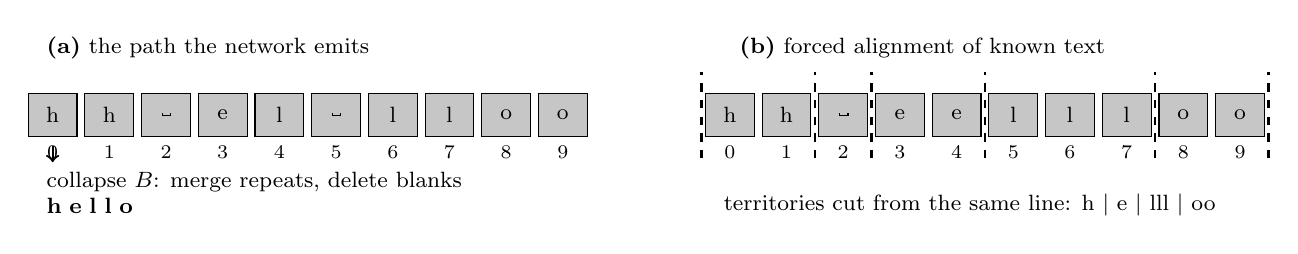
\begin{tikzpicture}[font=\footnotesize,
  cell/.style={draw,minimum width=6.2mm,minimum height=5.4mm,inner sep=0pt},
  blank/.style={cell,fill=gray!18},
  labl/.style={cell,fill=gray!45},
  brk/.style={draw,dashed,thick}]
% ---- left: emitted path -> collapse
\node[anchor=west] at (-0.2,3.35) {\textbf{(a)} the path the network emits};
\foreach \i/\s in {0/{h},1/{h},2/{\textvisiblespace},3/{e},4/{l},5/{\textvisiblespace},6/{l},7/{l},8/{o},9/{o}}{
  \ifx\s\textvisiblespace
    \node[blank] (a\i) at (\i*0.72,2.5) {\scriptsize$\varnothing$};
  \else
    \node[labl] (a\i) at (\i*0.72,2.5) {\s};
  \fi
}
\foreach \i in {0,...,9}{\node[font=\scriptsize,below] at (a\i.south) {\i};}
\node[anchor=west] at (-0.2,1.65) {collapse $B$: merge repeats, delete blanks};
\draw[->,thick] (0,2.1) -- (0,1.9);
\node[anchor=west] at (-0.2,1.35) {\textbf{h\;e\;l\;l\;o}};

% ---- right: known text -> forced alignment
\node[anchor=west] at (8.6,3.35) {\textbf{(b)} forced alignment of known text};
\foreach \i/\s in {0/{h},1/{h},2/{\textvisiblespace},3/{e},4/{e},5/{l},6/{l},7/{l},8/{o},9/{o}}{
  \ifx\s\textvisiblespace
    \node[blank] (b\i) at (8.6+\i*0.72,2.5) {\scriptsize$\varnothing$};
  \else
    \node[labl] (b\i) at (8.6+\i*0.72,2.5) {\s};
  \fi
}
\foreach \i in {0,...,9}{\node[font=\scriptsize,below] at (b\i.south) {\i};}
% character territories (blocks of steps assigned to one letter)
\draw[brk] (8.6-0.36,1.95) -- (8.6-0.36,3.05);
\draw[brk] (8.6+1*0.72+0.36,1.95) -- (8.6+1*0.72+0.36,3.05);
\draw[brk] (8.6+3*0.72-0.36,1.95) -- (8.6+3*0.72-0.36,3.05);
\draw[brk] (8.6+4*0.72+0.36,1.95) -- (8.6+4*0.72+0.36,3.05);
\draw[brk] (8.6+7*0.72+0.36,1.95) -- (8.6+7*0.72+0.36,3.05);
\draw[brk] (8.6+9*0.72+0.36,1.95) -- (8.6+9*0.72+0.36,3.05);
\node[anchor=west] at (8.6-0.2,1.35) {territories cut from the same line: h $\mid$ e $\mid$ lll $\mid$ oo};
\end{tikzpicture}
\caption{The two CTC operations used in this project. (a)~Collapsing the emitted path gives the transcription, so a line can be trained from its text alone with no character boundaries. (b)~Given the text, forced alignment finds the most probable block of time steps for each character; the dashed lines are the resulting territories, from which individual letter shapes are cut. Blank symbols are shaded.}
\label{fig:lit-ctc}
\end{figure}

Graves \emph{et al.}~\cite{graves2009} combined BiLSTM and CTC, reporting word accuracies of 74.1\,\% offline and 79.7\,\% online on IAM-derived data. Shi \emph{et al.}~\cite{shi2017} replaced the raw-pixel input by CNN features, naming the arrangement the convolutional recurrent neural network (CRNN). Puigcerver~\cite{puigcerver2017} showed on IAM that a CNN followed by BiLSTM layers matches costlier multidimensional recurrence, and the first-semester sources~\cite{ma2023,kumar2024,hemanth2022} agree.

\paragraph{Reported accuracies.}\label{sec:lit-acc} Quality is the character error rate (CER), the Levenshtein distance~\cite{levenshtein1966} between recognised and reference text divided by the reference length, or the word error rate (WER); this report uses character accuracy $1-\text{CER}$. Kizilirmak and Yanikoglu~\cite{kizilirmak2023}, whose CNN--BiLSTM--CTC network is closest to this one, report a best CER of 3.59\,\% and WER of 9.44\,\% on IAM, but only with lexicon-constrained decoding and test-time augmentation, so greedy decoding is worse. Word error rates run several times the CER because errors cluster inside words, and the accuracies above 95\,\% in the first-semester sources~\cite{yahya2021,ji2021,chen2023} are for isolated characters on clean data. Published work is also evaluated mostly on scanner images rather than on office photographs, which have uneven lighting, perspective, shadows and clutter, so pre-processing cannot be omitted.

\subsubsection{Image pre-processing and page segmentation}
\label{sec:lit-prep}

A photographed page must first become clean, separated line images; the first-semester sources~\cite{chen2023,hemanth2022} list normalisation, binarisation and line separation as standard.

A photograph records reflectance multiplied by lighting, so a lamp gradient or shadow changes the grey value of the paper itself, while \emph{binarisation} must decide for each pixel whether it is ink. Otsu's global method~\cite{otsu1979} picks the threshold $t^{*}$ maximising the between-class variance,
\begin{equation}
t^{*}=\arg\max_{t}\;\omega_{B}(t)\,\omega_{F}(t)\,\bigl[\mu_{B}(t)-\mu_{F}(t)\bigr]^{2},
\label{eq:lit-otsu}
\end{equation}
In Equation~\ref{eq:lit-otsu}, $\omega_B(t)$ and $\omega_F(t)$ are the fractions of pixels at or below, and above, $t$, with mean grey values $\mu_B(t)$ and $\mu_F(t)$. It needs no tuning but fails under uneven lighting, dropping strokes in dim areas or reading shadows as ink. \emph{Adaptive} methods threshold each pixel against a local mean and standard deviation~\cite{sauvola2000} or an integral image~\cite{bradley2007}; flat-field correction, dividing the image by a blurred copy of itself, flattens a multiplicative gradient. The summed-area table of Crow~\cite{crow1984} makes local means cheap, any rectangle sum needing four look-ups.

Ink pixels are grouped into \emph{connected components} by the two-pass labelling of Rosenfeld and Pfaltz~\cite{rosenfeld1966}; their heights give a typical character height, so thresholds in character heights are independent of camera resolution and handwriting size. Skew is found by rotating through trial angles and keeping the most sharply peaked row-wise ink histogram, the projection-profile method of Postl~\cite{postl1986} \mustdo{confirm the exact title and page range of the Postl 1986 ICPR reference, or replace it with Baird 1987 if that is the source preferred; the page range was left out of the bibliography rather than guessed.}. Lines come from gaps in that profile, which assumes straight lines, or from chaining neighbouring components, which tolerates drifting baselines and diagrams. Printed ruling lines glue letters together and must be removed without deleting the strokes crossing them. These steps are described for scanned documents rather than for a camera, desk background, ruled paper and diagrams together.

\subsubsection{Writer identification and style}
\label{sec:lit-writer}

Writer identification asks which member of a known set wrote a sample. The proposal grounded its target in the signature classification of Agduk and Aydemir~\cite{agduk2022}, who compared transfer-learning CNNs; signatures are short and practised, whereas this system must identify the writer of running text while reading it. Bulacu and Schomaker~\cite{bulacu2007} are \emph{text independent}, comparing histograms of contour direction and curvature against those of characteristic letter shapes; slant, x-height, stroke width, spacing and joined-letter frequency also describe style. A CNN can instead be trained on the images: FragNet~\cite{he2020} classifies small fragments and pools the evidence.

Two cautions affect the project. A classifier trained on ink can rely on cues a machine cannot reproduce: stroke thickness and ink density follow the writer's pen and pressure, whereas a robot draws at constant width. Most of this work uses hundreds of writers, whereas this closed set of thirteen has about one and a half thousand text lines, and test partitions that share pages with training data inflate accuracy.

\subsubsection{Handwriting synthesis and pen-path generation}
\label{sec:lit-synth}

\emph{Neural sequence generators} are trained on recorded pen trajectories: Graves~\cite{graves2013} conditioned an LSTM on the text through a soft attention window to predict the next pen offset and pen-up probability, which needs hundreds to thousands of recorded lines that photographs of a few pages cannot supply. Pretrained image generators such as the generative adversarial network of Kang \emph{et al.}~\cite{kang2020} need less data per writer, but produce rasters and give no control of slant, size or spacing. \emph{Exemplar} (glyph-based) methods are the alternative: Haines \emph{et al.}~\cite{haines2016} assemble glyphs from an annotated sample with learned spacing, thickness and pressure, so a few pages per writer suffice and the letterforms are the writer's own. Forced alignment of the transcription with a recogniser's output (Section~\ref{sec:lit-nn}) extracts those glyphs without hand-drawn boundaries.

\emph{Thinning} reduces a stroke to a one-pixel centre line without breaking connectivity; Zhang and Suen~\cite{zhang1984} delete boundary pixels in two alternating sub-iterations. The Douglas--Peucker algorithm~\cite{douglas1973} then simplifies the traced line, recursively keeping the point farthest from the chord while its distance exceeds a tolerance $\varepsilon$; the first-semester report noted it is not guaranteed optimal.

\subsubsection{Robotic writing and linear motion}
\label{sec:lit-robot}

The first-semester study identified three robot topologies~\cite{teikari2016}. A \emph{Cartesian} (gantry) system moves along two perpendicular linear axes: it is simple, its kinematics are the identity and it covers a flat page naturally. \emph{Serial-chain} arms reach further but need inverse kinematics and accumulate joint errors; \emph{parallel} robots are stiff and precise but have a small workspace. Belt, rack-and-pinion and ball-screw actuators are used in handwriting systems for durability and low cost~\cite{acarnley2002}.

Most such systems use stepper motors, which turn by a fixed angle for every pulse; a driver converts the pulse (STEP) and direction level (DIR) into winding currents, and microstepping gives finer positions. Acarnley~\cite{acarnley2002} treats open-loop stepping, torque--speed limits and controlled acceleration to avoid lost steps. Because position follows from counting pulses, error does not accumulate if commanded positions become integer step counts from a known reference. Bresenham's algorithm~\cite{bresenham1965}, from digital plotters, interleaves the two axes of a line in integer arithmetic, an error accumulator deciding when the slower axis steps, so the deviation never exceeds one step.

The proposal used Teikari's analysis~\cite{teikari2016} to set about four seconds per character, the 0.3\,mm gantry error of Huang and Xiong~\cite{huang2024} as the basis of the 0.5\,mm limit of R5, and the roughly 85\,\% accuracy derived from Babushkin \emph{et al.}~\cite{babushkin2025} for R1. None shows how a robot would reproduce an \emph{identified} person's style from a photograph.

\subsubsection{Embedded deployment and shortcomings of the literature}
\label{sec:lit-embedded}

Executing all processing on a single-board computer (SBC) makes every algorithm's cost matter. Sze \emph{et al.}~\cite{sze2017} stress that multiply--accumulate operations and the memory for weights and activations determine time and energy on a constrained processor, and that convolutions dominate. Most research relies on large frameworks, so the algorithms are never exposed~\cite{chen2023}.

Four shortcomings follow. First, recognition, writer identification, synthesis and robotics are studied in isolation, with no complete system from a photographed page to a drawn one. Second, embedded deployment is rarely demonstrated, and then through frameworks. Third, reported accuracies depend on benchmark conditions (lexicon, scanner images, shared writers or pages) unlike a photograph. Fourth, the generation literature needs recorded trajectories or large pre-training and evaluates output as an image, whereas this project must evaluate output a machine can draw with a constant-width pen.

\subsection{Application of the background to this project}
\label{sec:lit-application}

\subsubsection{Reading and identification (R2, R4)}

Cursive writing cannot be segmented reliably and the labels are line transcriptions, so a line-level recogniser trained with CTC~\cite{graves2006} was adopted and FU\,2.2 (character separation) became separation into \emph{lines}.
The architecture follows the CNN--BiLSTM--CTC pattern~\cite{shi2017,puigcerver2017,kizilirmak2023} with about 3.36 million parameters; decoding is greedy, because lexicon decoding needs corpora the project does not have (Sections~\ref{sec:textrec} and~\ref{sec:results}).
For writer identification a learned CNN on text lines was chosen over hand-crafted statistics~\cite{bulacu2007} or fragment pooling~\cite{he2020}, since the recogniser's features could be reused and accuracy measured directly.
Following Section~\ref{sec:lit-writer}, two classifiers of the same architecture were built: one on real photographed ink, one on lines thinned and redrawn at constant width, which removes thickness and pressure cues and matches the gantry.
The second was needed because the first, almost perfect on real handwriting, identified only 28\,\% of the machine's drawn lines (Section~\ref{sec:writerid}).
Both are closed-set decisions: they address R2 and the storage requirement of R6 but cannot report an unknown writer (Section~\ref{sec:dis-failure}).

\subsubsection{Reproduction (R1, R3, R5, R6)}

Neural generators need pen recordings the project does not have, and image generators produce rasters without parametric control, so an exemplar approach after Haines \emph{et al.}~\cite{haines2016} was adopted.
Glyphs are harvested from each writer's pages: the recogniser aligns the known transcription with the line (Figure~\ref{fig:lit-ctc}b), the ink is cut into letter territories, thinned~\cite{zhang1984}, traced, simplified~\cite{douglas1973}, normalised to the x-height and de-slanted; the glyphs and style statistics form a \emph{style profile} stored as a file.
Synthesis places glyphs with the writer's slant, spacing and random variation; the best of several candidates is kept by a combined score of legibility and writer-classifier confidence.
The scoring networks also perform the selection and so cannot be an independent verdict (Sections~\ref{sec:synthesis} and~\ref{sec:results}).

A Cartesian gantry with stepper motors was adopted, since position follows from step counts, the only practical route to 0.5\,mm without position sensors.
Pen paths in millimetres become G-code, which a program converts to absolute integer step counts, interleaving the axes with Bresenham's algorithm~\cite{bresenham1965} and reading the limit switches before every step; the step resolution is 12.5\,$\mu$m against the 0.5\,mm limit of R5 (Section~\ref{sec:gantry}).
Resolution is not accuracy: belt stretch, backlash, home-switch repeatability and pen compliance determine the true error, and none was measured, so R5 remains unassessed in Section~\ref{sec:results}.

\subsubsection{Embedded execution and the contribution}

Following Sze \emph{et al.}~\cite{sze2017}, the networks' cost was analysed: about $4.2\times10^{9}$ multiply--accumulate operations and 13.4\,MB of weights per recogniser pass, 91\,\% of the arithmetic being convolution.
Inference of both networks was therefore written from first principles in Python, without a neural-network framework, and agrees with the training implementation to about $10^{-5}$ in log-probability (Section~\ref{sec:textrec}).
Recognition met the 25\,ms allowance of R4 at 8.86\,ms per character, but page segmentation took 35 to 57\,s against the roughly 2\,s the requirement leaves, so R4 fails on segmentation rather than on the network (Section~\ref{sec:results}).
The contribution is therefore a complete pipeline from photograph to pen strokes, implemented from first principles in one language.
